\chapter{Анализ самоорганизующихся низкоскоростных сетей передачи данных} \label{ch1}

% не рекомендуется использовать отдельную section <<введение>> после лета 2020 года
%\section{Введение. Сложносоставное название первого параграфа первой главы для~демонстрации переноса слов в содержании} \label{ch1:intro}

В данной главе рассматриваются ключевые аспекты самоорганизующихся низкоскоростных одноранговых (\textit{англ.} peer-to-peer, \textit{далее} — P2P) сетей с мобильными узлами (\textit{англ.} mobile nodes, \textit{в дальнейшем} — абонентами), работающими в условиях ограниченной пропускной способности радиоканала (от 32 бит/с до 37 кбит/с) и высокой мобильности участников (до 60 км/ч). Основное внимание уделяется проблемам децентрализованных сетей, алгоритмам маршрутизации и методам оптимизации энергопотребления.

В параграфе \ref{ch1:sec1} анализируются особенности самоорганизующихся сетей, включая принципы работы P2P-сетей (\textit{англ.} Peer-to-Peer networks) и специфику низкоскоростных беспроводных соединений. Параграф \ref{ch1:sec2} посвящен обзору современных алгоритмов маршрутизации и методов энергосбережения.

\section{Особенности самоорганизующихся сетей} \label{ch1:sec1}

\subsection{Децентрализованные P2P-сети: принципы функционирования} \label{ch1:sec1:subsec1}

Одноранговые (P2P, peer-to-peer) сети представляют собой распределенные вычислительные системы, в которых отсутствует централизованный управляющий сервер, а каждый узел (peer) может выполнять функции как клиента, так и сервера \cite{tanenbaum2011computer}.

Основные принципы функционирования P2P-сетей включают:

\begin{itemize}
\item Децентрализованную архитектуру управления
\item Равноправие всех участников сети (абонентов)
\item Автономность работы отдельных абонентов
\item Динамическую адаптацию к изменяющейся топологии
\end{itemize}

Ключевые преимущества P2P-сетей, согласно исследованиям \cite{schollmeier2002peer}, включают:

\begin{enumerate}
\item Повышенную отказоустойчивость за счет отсутствия единой точки отказа
\item Горизонтальную масштабируемость при добавлении новых абонентов
\item Эффективное использование распределенных ресурсов
\item Снижение нагрузки на каналы связи за счет локальной маршрутизации
\end{enumerate}

Однако в условиях низкоскоростных мобильных сетей возникают специфические проблемы, связанные с:

\begin{itemize}
\item Нестабильностью соединений
\item Ограниченной пропускной способностью
\item Высокой латентностью
\item Энергетическими ограничениями мобильных устройств
\end{itemize}

Для математического описания вероятности успешного соединения между абонентами в таких условиях может быть использована следующая модель:

\begin{equation}
\label{eq:connection-prob}
P_{\text{success}} = e^{-\alpha \frac{d_{ij}}{R}}, \quad \alpha \in [0.1, 0.5]
\end{equation}

где:
\begin{itemize}
\item $P_{\text{success}}$ - вероятность успешной передачи данных;
\item $d_{ij}$ - расстояние между абонентами $i$ и $j$;
\item $R$ - максимальный радиус устойчивой связи;
\item $\alpha$ - коэффициент затухания сигнала, зависящий от характеристик среды передачи.
\end{itemize}

\begin{figure}[h]
\centering
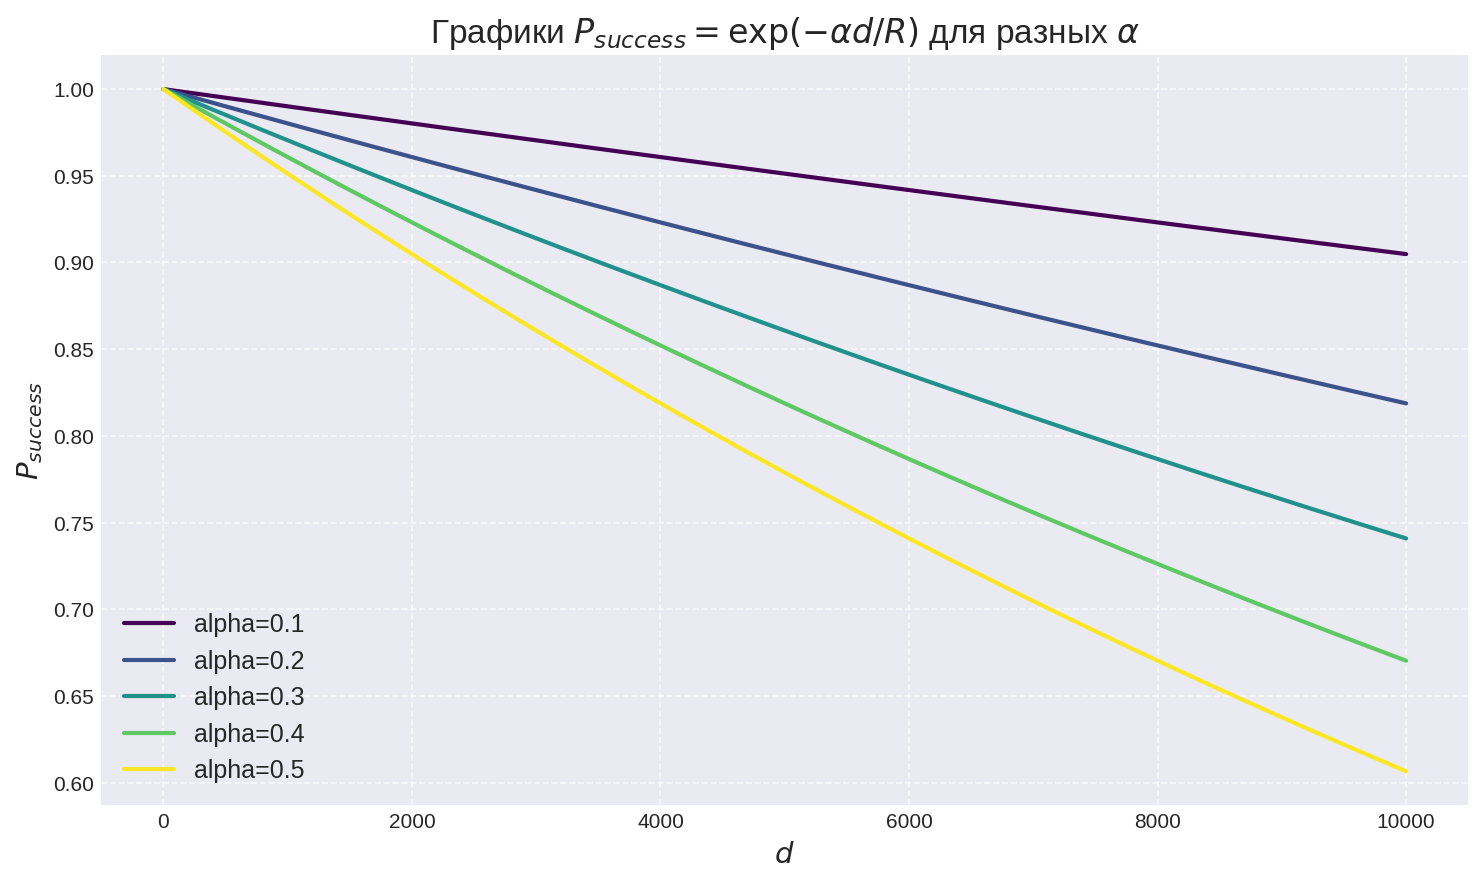
\includegraphics[width=0.8\textwidth]{exp.png}
\caption{Зависимость вероятности успешной передачи $P_{\text{success}}$ от относительного расстояния $d_{ij}/R$ для различных значений коэффициента затухания $\alpha$}
\label{fig:exp_plot}
\end{figure}

Как видно из графика на Рис.~\ref{fig:exp_plot}, вероятность успешной передачи данных экспоненциально уменьшается с ростом расстояния между абонентами. При этом:
\begin{itemize}
\item Для $\alpha = 0.1$ (наилучшие условия) вероятность остается высокой ($>80\%$) даже на расстояниях $0.8R$
\item Для $\alpha = 0.5$ (худшие условия) вероятность падает ниже $60\%$ уже на расстоянии $0.5R$
\item Критическое расстояние ($P_{\text{success}} \leq 10\%$) достигается при $d_{ij}/R \approx 2.3$ для $\alpha=0.5$
\end{itemize}

Данная модель демонстрирует экспоненциальную зависимость качества соединения от расстояния между абонентами \cite{goldsmith2005}, что актуально и для мобильных сетей с динамически изменяющейся топологией.

\begin{figure}[ht!] 
	\center
	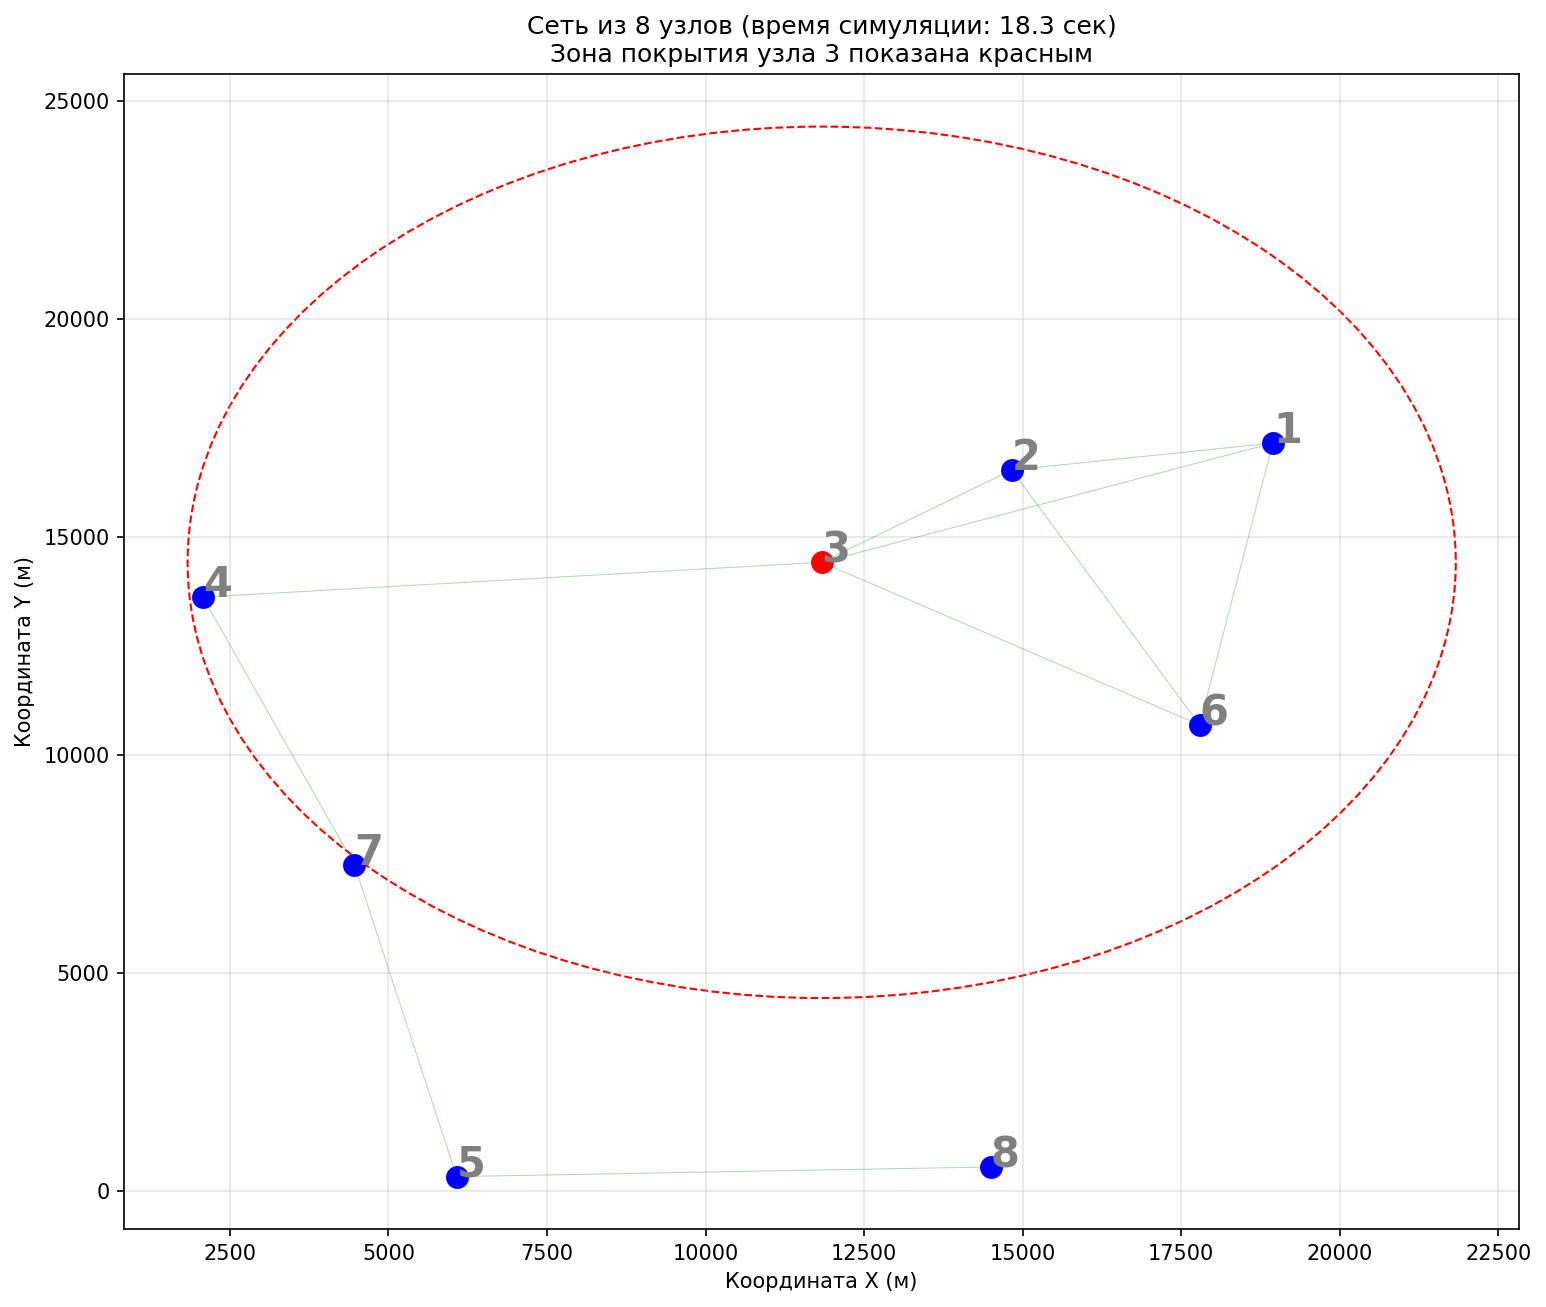
\includegraphics [scale=0.6] {my_folder/images//network_topology}
	\caption{Пример топологии самоорганизующейся сети с мобильными абонентами} 
	\label{fig:network_topology}  
\end{figure}

На \firef{fig:network_topology} изображена топология самоорганизующейся сети с мобильными абонентами


\subsection{Проблемы низкоскоростных беспроводных сетей} \label{ch1:sec1:subsec2}

\begin{enumerate}
    \item \textbf{Нестабильность соединений}:
    \begin{itemize}
        \item Динамическое изменение качества связи при движении абонентов (типичный радиус действия составляет $\leq 10$ км)
        \item Частые разрывы соединений, вызванные:
        \begin{itemize}
            \item физическими препятствиями
            \item интерференцией сигналов
            \item изменением условий распространения радиоволн
        \end{itemize}
    \end{itemize}
    
    \item \textbf{Потери данных при передаче}:
    \begin{itemize}
        \item Уровень потерь пакетов достигает 22\% в экстремальных условиях \cite{zuniga2004analyzing}
        \item Необходимость механизмов повторной передачи данных, приводящая к:
        \begin{itemize}
            \item увеличению нагрузки на сеть
            \item росту энергопотребления абонентов
        \end{itemize}
    \end{itemize}
    
    \item \textbf{Задержки передачи и синхронизации}:
    \begin{itemize}
        \item Время синхронизации между абонентами превышает 5 с при скорости передачи 32 бит/с
        \item Накопительный эффект задержек, проявляющийся:
        \begin{itemize}
            \item в многоабонентных конфигурациях
            \item при каскадном соединении устройств
        \end{itemize}
    \end{itemize}
    
    \item \textbf{Динамическое изменение топологии сети}:
    \begin{itemize}
        \item Необходимость частого перерасчета маршрутов, вызванная:
        \begin{itemize}
            \item перемещением абонентов
            \item изменением качества каналов связи
        \end{itemize}
        \item Проблемы поддержания устойчивых маршрутов передачи данных
    \end{itemize}
    
    \item \textbf{Физические эффекты}:
    \begin{itemize}
        \item Допплеровский сдвиг частот ($\pm 110$ Гц при несущей частоте 862 МГц)
        \item Многолучевое распространение сигналов, приводящее к:
        \begin{itemize}
            \item интерференционным искажениям
            \item временным рассеяниям сигнала
        \end{itemize}
        \item Замирания сигнала (фединг) различных типов:
        \begin{itemize}
            \item релеевский
            \item рициановский
        \end{itemize}
    \end{itemize}
\end{enumerate}


\section{Обзор существующих алгоритмов маршрутизации} \label{ch1:sec2} 


\subsection{Протоколы для мобильных ad-hoc сетей (MANET)} \label{ch1:sec2:subsec1}
Мобильные самоорганизующиеся сети (Mobile Ad-hoc Networks, MANET) требуют специальных адаптивных протоколов маршрутизации, учитывающих их динамическую природу. Согласно исследованиям \cite{perkins2003performance}, ключевые аспекты проектирования таких протоколов включают:

\begin{enumerate}
    \item \textbf{Учет динамики изменения топологии}:
    \begin{itemize}
        \item Прогнозирование позиций абонентов на основе кинематической модели:
        \begin{equation}
        \label{eq:node_movement}
        \begin{cases} 
        x_i(t + \Delta t) = x_i(t) + v_i \cos\theta_i \Delta t \\
        y_i(t + \Delta t) = y_i(t) + v_i \sin\theta_i \Delta t 
        \end{cases}
        \end{equation}
        где:
        \begin{itemize}
            \item $x_i(t)$, $y_i(t)$ - координаты абонента $i$ в момент времени $t$
            \item $v_i$ - скорость перемещения абонента
            \item $\theta_i$ - направление движения
            \item $\Delta t$ - временной интервал прогнозирования
        \end{itemize}
        \item Адаптация к частоте изменений топологии (до 3 изменений/сек \cite{lee2016survey})
    \end{itemize}
    
    \item \textbf{Оценка качества связи}:
    \begin{itemize}
        \item Мониторинг параметров канала:
        \begin{itemize}
            \item Уровень сигнала (RSSI)
            \item Вероятность ошибок (BER)
            \item Пропускная способность
        \end{itemize}
        \item Использование метрик качества для выбора оптимального маршрута
    \end{itemize}
    
    \item \textbf{Энергоэффективность}:
    \begin{itemize}
        \item Оптимизация энергопотребления по метрикам:
        \begin{equation}
        E_{route} = \sum_{k=1}^{n} E_k^{trans} + E_k^{rec}
        \end{equation}
        где $E_k^{trans}$ и $E_k^{rec}$ - энергия передачи и приема на $k$-м абоненте маршрута
        \item Реализация механизмов энергосбережения \cite{akylidiz2002survey}
    \end{itemize}
\end{enumerate}

Основные классы протоколов MANET \cite{gupta2015routing}:
\begin{itemize}
    \item Табличные (DSDV, OLSR)
    \item Реактивные (AODV, DSR)
    \item Гибридные (ZRP)
    \item Географические (GPSR)
\end{itemize}


\subsection{Методы оптимизации энергопотребления} \label{ch1:sec2:subsec2}

Оптимизация энергопотребления является критически важной задачей для низкоскоростных беспроводных сетей, особенно в условиях ограниченных энергоресурсов мобильных устройств \cite{chen2014energy}. Основные методы энергосбережения включают:

\begin{enumerate}    
    \item \textbf{Приоритезация сообщений}:
    \begin{itemize}
        \item Многофакторная оценка приоритета передаваемых данных:
        \begin{equation}
        \label{eq:priority}
        Priority = \alpha \cdot \frac{S_{msg}}{S_{max}} + (1 - \alpha) \cdot \frac{A_{msg}}{A_{max}} + \beta \cdot Q_{link}
        \end{equation}
        где:
        \begin{itemize}
            \item $S_{msg}$ - размер сообщения
            \item $S_{max}$ - максимальный размер пакета
            \item $A_{msg}$ - возраст данных
            \item $A_{max}$ - максимальный допустимый возраст
            \item $Q_{link}$ - качество канала связи (0..1)
            \item $\alpha$, $\beta$ - весовые коэффициенты
        \end{itemize}
    \end{itemize}
    
    \item \textbf{Оптимизация служебного трафика}:
    \begin{itemize}
        \item Адаптивное регулирование интервалов сканирования:
        \begin{equation}
        \label{eq:scan_interval}
        T_{scan} = T_{min} + (T_{max} - T_{min}) \cdot e^{-\lambda t}, \quad T_{scan} \in [5, 60]\, \text{с}
        \end{equation}
        где $\lambda$ - коэффициент адаптации, $t$ - время работы сети
        \item Использование механизмов прогнозирования для уменьшения служебных сообщений \cite{wang2015energy}
    \end{itemize}
\end{enumerate}

Экспериментальные исследования \cite{kim2017efficient} показывают, что применение данных методов позволяет достичь:
\begin{itemize}
    \item Снижения энергопотребления на 35-40\%
    \item Увеличения времени работы сети на 25-30\%
    \item Сохранения приемлемого качества обслуживания QoS (англ. Quality of Service)
\end{itemize}


\section{Выводы} \label{ch1:conclusion}

Проведенный анализ особенностей самоорганизующихся низкоскоростных сетей передачи данных позволяет сформулировать следующие основные выводы:

\begin{enumerate}
    \item \textbf{Особенности архитектуры}:
    \begin{itemize}
        \item Децентрализованные P2P-сети демонстрируют высокую отказоустойчивость за счет отсутствия единой точки отказа \cite{abdrabou2008position}
        \item Для работы в условиях низкой пропускной способности (32-64 бит/с) требуются специализированные алгоритмы маршрутизации
        \item Мобильность абонентов (до 60 км/ч) существенно осложняет поддержание стабильных соединений
    \end{itemize}
    
    \item \textbf{Ключевые проблемы}:
    \begin{itemize}
        \item Нестабильность соединений, вызванная:
        \begin{itemize}
            \item динамическим изменением топологии
            \item эффектом Допплера (±110 Гц при 862 МГц)
        \end{itemize}
        \item Потери данных достигают 22\% при скорости передачи 32 бит/с \cite{zuniga2004analyzing}
        \item Задержки синхронизации между абонентами превышают 5 секунд
    \end{itemize}
    
    \item \textbf{Алгоритмы маршрутизации}:
    \begin{itemize}
        \item Существующие протоколы (AODV, DSR) требуют модификации для экстремальных условий
        \item Необходима разработка гибридных алгоритмов, сочетающих:
        \begin{itemize}
            \item реактивную маршрутизацию
            \item прогнозирование позиций абонентов
            \item учет энергоресурсов
        \end{itemize}
    \end{itemize}
    
    \item \textbf{Ограничения масштабируемости}:
    \begin{itemize}
        \item Максимальное число абонентов в сети ограничено пропускной способностью канала
        \item Экспериментальные данные \cite{li2013capacity} показывают:
        \begin{equation}
        N_{max} = \left\lfloor \frac{B \cdot \eta}{R_{min} \cdot (1 + \alpha)} \right\rfloor
        \end{equation}
        где:
        \begin{itemize}
            \item $B$ - полоса пропускания
            \item $\eta$ - коэффициент использования канала
            \item $R_{min}$ - минимальная скорость передачи
            \item $\alpha$ - коэффициент служебного трафика
        \end{itemize}
        \item При типичных параметрах $N_{max} \in [31, 50]$ абонентов
    \end{itemize}
\end{enumerate}
